\Chapter{Esperimenti}


\Section{Introduzione}
Sono stati condotti diversi esperimenti, cercando di variare gli aspetti della configurazione del modello e del processo di addestramento, al fine di ottimizzare le prestazioni nella segmentazione delle immagini mammografiche. Si è cercato di \textbf{cambiare gli iperparametri uno alla volta}, mantenendo costanti gli altri, per isolare l'impatto di ciascuna modifica. 

Lo sviluppo di un sistema di segmentazione automatica efficace richiede non solo un’adeguata progettazione architetturale, ma anche un attento processo di \textbf{ottimizzazione sperimentale}, che tenga conto delle molteplici variabili che influenzano l’apprendimento del modello. In questo capitolo viene descritto in dettaglio il percorso iterativo seguito, che ha portato a una \textbf{progressiva evoluzione del modello} fino a raggiungere \textbf{performance soddisfacenti}.

\Subsection{Nota sulle Valutazioni}
Nei primi \textbf{16 esperimenti}, la valutazione sul \textbf{test set} è stata effettuata utilizzando le \textbf{immagini trasformate}, ovvero mantenendo le dimensioni e le modifiche introdotte durante il preprocessing (incluso il resize). A partire dall'esperimento \textbf{17}, invece, è stata applicata una \textbf{trasformazione inversa} (in particolare il resize inverso) alle ground truth, riportandole alle dimensioni originali. Questo ha permesso una valutazione più corretta e realistica delle performance, evitando possibili distorsioni dovute alle trasformazioni di preprocessing.

\begin{table}[!ht]
    \begin{center}
    \begin{NiceTabular}{rrr}[rules/color={gray!90},rules/width=1pt]
        \CodeBefore
        \rowcolors{1}{black!5}{}
        \rowcolors{3}{blue!5}{}
        \Body
        \toprule
        \textbf{EXP} & \textbf{Architettura} & \textbf{Parametri Chiave} \\
        \midrule
        1-3 & U-Net 3D & Canali [16,32,64,128] \\
        4-10 & U-Net 3D & Canali [16,32,64,128,256] \\
        12,13 & SliceU-Net 2D & Approccio 2D slice-based \\
        14-21 & U-Net 3D & Varianti profondità/canali \\
        20 & Attention U-Net 3D & Meccanismo di attention \\
        \bottomrule
    \end{NiceTabular}
\end{center}
    \caption{Configurazioni principali dei modelli sperimentali con architetture e parametri chiave.}
    \label{tab:config_modelli}
\end{table}




\Section{Impostazione degli Esperimenti}

Gli esperimenti sono stati condotti in \textbf{maniera incrementale}, seguendo una filosofia di \hlight{ottimizzazione guidata da evidenze}, nella quale ciascuna modifica introdotta agli iperparametri o alla pipeline di preprocessing è stata motivata da osservazioni emerse negli esperimenti precedenti. Tutte le prove sono state \textbf{documentate} e \textbf{monitorate} con precisione.

Per garantire la coerenza e individuare possibili problemi, è stato anche necessario implementare un sistema di \hlight{debugging interno} tramite Python, includendo \textbf{stampe delle dimensioni dei tensori nei momenti chiave} del forward pass e salvataggi intermedi delle immagini durante il training. Questo approccio ha \hlight{permesso di identificare rapidamente errori legati a mismatch dimensionali, problemi nella gestione della normalizzazione, o trasformazioni incoerenti nei dati di input/output.}

\Section{Evoluzione Architetturale e Tuning degli Iperparametri}

Il \textbf{primo esperimento} \ref{tab:exp1_config} ha costituito la \textbf{base di partenza}, con una configurazione \textbf{standard della rete U-Net tridimensionale}, con \textbf{4 blocchi convoluzionali} (\texttt{channels: [16, 32, 64, 128]}), \textbf{normalizzazione batch}, e un \textbf{resize uniforme} applicato a tutte le immagini. Con questa configurazione, è stato ottenuto un \hlight{Dice score sul test set pari a 0.7894}.

\begin{table}[H]
    \begin{center}
        \begin{NiceTabular}{rc}[rules/color={gray!90},rules/width=1pt]
            \CodeBefore
            \rowcolors{1}{black!5}{}
            \rowcolors{3}{blue!5}{}
            \Body
            \toprule
            \textbf{Parametro}      & \textbf{Valore}                                \\
            \midrule
            \textbf{Architettura} & U-Net 3D standard con 4 blocchi convoluzionali \\
            \textbf{Canali} & [16, 32, 64, 128] \\
            \textbf{Normalizzazione} & Batch normalization \\
            \textbf{Resize} & Uniforme su tutte le immagini \\
            \textbf{Dice score (test set)} & 0.7894 \\
            \bottomrule
        \end{NiceTabular}
    \end{center}
	\caption{Configurazione del primo esperimento (baseline) con architettura U-Net 3D e risultati ottenuti.}
	\label{tab:exp1_config}
\end{table}


Il \textbf{passo successivo} ha previsto un \textbf{aumento del learning rate} dell’ottimizzatore \textbf{Adam}, passando da \textbf{0.0005} a \textbf{0.005}. Questo semplice cambiamento ha prodotto un \hlight{incremento della metrica di circa +1.17\%,} suggerendo che la rete era in grado di \hlight{convergere più rapidamente in presenza di un gradiente iniziale più marcato}. Da qui è emersa l’intuizione che la rete potesse beneficiare anche di una \hlight{maggiore profondità}: il \textbf{terzo} e il \textbf{quarto} esperimento \ref{tab:exp3-4_results} \hlight{hanno confermato questa ipotesi, mostrando miglioramenti crescenti in validazione e test} con l’introduzione di un ulteriore blocco (\texttt{channels: [16, 32, 64, 128, 256]}), fino a raggiungere \hlight{0.8597 sul test set} e \hlight{0.8569 sul validation set}.

\begin{table}[H]
    \centering
	\begin{NiceTabular}{rc}[rules/color={gray!90},rules/width=1pt]
		\CodeBefore
		\rowcolors{1}{black!5}{}
		\rowcolors{3}{blue!5}{}
		\Body
		\toprule
		\textbf{Parametro} & \textbf{Valore} \\
		\midrule
		\textbf{Architettura} & U-Net 3D profonda con 5 blocchi convoluzionali \\
		\textbf{Canali} & [16, 32, 64, 128, 256] \\
		\textbf{Normalizzazione} & Batch normalization \\
		\textbf{Dice score (test)} & 0.8597 \\
		\textbf{Dice score (validazione)} & 0.8569 \\
		\bottomrule
	\end{NiceTabular}
	\caption{Risultati degli esperimenti 3-4 con architettura U-Net 3D più profonda. L'aggiunta di un quinto blocco convoluzionale ha portato a significativi miglioramenti nelle metriche.}
	\label{tab:exp3-4_results}
\end{table}

A partire dal \textbf{quinto esperimento} \ref{tab:exp5_comparative} è stata esplorata una \textbf{combinazione di modifiche strutturali}, tra cui il passaggio da \textbf{Adam} ad \hlight{AdamW}, il cambiamento della \textbf{normalizzazione} da \textbf{Batch} a \hlight{Instance} e l’utilizzo di una \textbf{loss} \textbf{composita} (\hlight{Focal} + \hlight{Dice} \hlight{Loss}), ciascuna ponderata per gestire in modo bilanciato gli squilibri tra le classi. Questa configurazione ha prodotto \hlight{ottimi risultati in validazione (0,8623) e (0,8597) sul test set}.
\begin{table}[H]
    \centering
    \begin{NiceTabular}{rl}[rules/color={gray!90},rules/width=1pt]
        \CodeBefore
        \rowcolors{1}{black!5}{}
        \rowcolors{3}{blue!5}{}
        \Body
        \toprule
        \textbf{Componente} & \textbf{Modifica} \\
        \midrule
        \textbf{Ottimizzazione} & Sostituzione Adam → AdamW \\
        \textbf{Normalizzazione} & Batch → Instance \\
        \textbf{Loss function} & Dice → DiceFocal ($\lambda$ =0.7/0.3) \\
        \textbf{Metriche} & $\Delta$ Valid +3.1\%, $\Delta$ Test +0.32\% \\
        \textbf{Risultati} & Valid: 0.8623, Test: 0.8597 \\
        \bottomrule
    \end{NiceTabular}
    \caption{Analisi comparativa delle modifiche introdotte dall'EXP 5. Tutti i cambiamenti hanno contribuito al miglioramento delle performance.}
    \label{tab:exp5_comparative}
\end{table}


Nei \textbf{successivi esperimenti}, si è indagata ulteriormente la sensibilità del modello al \textbf{learning rate}, che era stato inizialmente portato troppo in basso (\texttt{0.0001}). Ripristinando un valore intermedio (\texttt{0.001}), il \hlight{Dice score sul test è aumentato di oltre il 3\%.} Parallelamente, l’introduzione di una strategia di \hlight{learning rate scheduling  (LinearWarmupCosineAnnealingLR)} \ref{fig:learning_rate_scheduling} ha portato a \hlight{miglioramenti più modesti ma stabili}.

\begin{figure}[H] 
  	\centering 
 	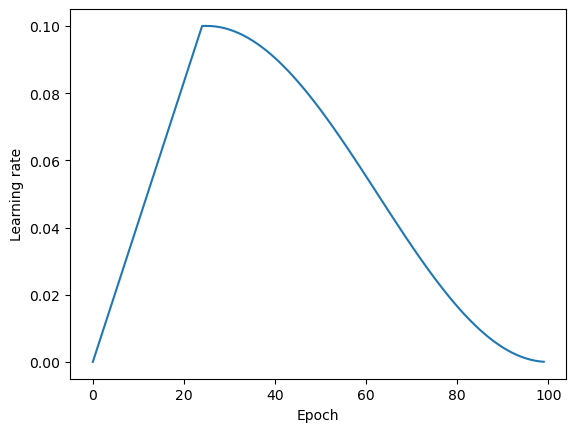
\includegraphics[width=.6\textwidth]{images/2025-07-12-11-28-31.png} 
    \caption{Andamento del learning rate durante il training, con warmup iniziale e successiva discesa coseno.}
    \label{fig:learning_rate_scheduling}
 \end{figure} 



 


Una seconda linea di sperimentazione ha riguardato il \textbf{trattamento dimensionale} delle immagini. Portando la dimensione da \textbf{384x384} a \hlight{512x512}, si è osservato un ulteriore \hlight{miglioramento della metrica}. Al contrario, strategie basate esclusivamente sul \textbf{padding}, o su un \textbf{mix di resize e padding}, hanno avuto un effetto \hlight{negativo} sulle performance, portando a un crollo significativo della metrica nel \textbf{nono} e \textbf{decimo} esperimento fino a \hlight{0.7576 sul test set} e \hlight{0.0816 in validazione}. 

\begin{table}[H]
    \centering
    \begin{NiceTabular}{rccc}[rules/color={gray!90},rules/width=1pt]
        \CodeBefore
        \rowcolors{1}{black!5}{}
        \rowcolors{3}{blue!5}{}
        \Body
        \toprule
        \textbf{Configurazione} & \textbf{Dimensione} & \textbf{Test Dice} & \textbf{Valid Dice} \\
        \midrule
        \textbf{Baseline} & 384×384 & 0.7894 & 0.7920 \\
        \rowcolor{green!5}
        \textbf{Full Resize} & 512×512 & \textbf{0,8878} & \textbf{0,8934} \\
        \rowcolor{red!5}
        \textbf{Solo Padding} & 512×512 & 0.7576 & 0.8160 \\
        \textbf{Mix Strategie} & Variabile & 0,8857 &  0,8848 \\
        \bottomrule
    \end{NiceTabular}
    \caption{Confronto sistematico degli approcci dimensionali. I valori mostrano come il resize completo produca i migliori risultati, mentre il padding peggiora le performance.}
    \label{tab:dimension_comparison}
\end{table}


\Section{Strategia Alternativa: Approccio 2D e Architettura SliceUNet}

In seguito a questi risultati, è stata sperimentata una \hlight{nuova strategia}, volta a esplorare un \hlight{approccio 2D} invece che 3D. Questo ha richiesto l’adozione di una \textbf{ROI size} di tipo \textbf{(512, 512, 1)}, accompagnata da una trasformazione \texttt{RandSpatialCropSamplesd} e da un’opportuna gestione del padding. Per rendere l’intera pipeline compatibile con questo formato, è stata definita un’architettura \hlight{SliceUNet personalizzata}, progettata per operare su \textbf{singole slice bidimensionali} mantenendo il supporto volumetrico per \textbf{l’aggregazione del risultato finale}.

\begin{code}{python}
class SliceUNet(nn.Module):
    def __init__(self, in_channels, out_channels, 
                channels, norm, strides, spatial_dims=2):
        super(SliceUNet, self).__init__()
        self.Unet2D = monai.networks.nets.UNet(
            spatial_dims=spatial_dims,
            in_channels=in_channels,
            out_channels=out_channels,
            channels=channels,
            strides=strides,
            norm= norm,
        )
    def forward(self, x):
        x = self.Unet2D(x[...,0]) 

        return x[..., None]
\end{code}



I primi esperimenti con \textbf{SliceUNet} hanno ottenuto \hlight{risultati interessanti}: partendo da \textbf{0.628}, si è passati a \hlight{0.7808, in test}, modificando la strategia di preprocessing da \textbf{padding} a \hlight{resize}. Tuttavia, nonostante \textbf{l’eleganza} e la \textbf{semplicità computazionale} di questo approccio, i risultati \hlight{non hanno raggiunto i livelli di accuratezza ottenibili con la versione 3D}.

\Section{Ritorno all’approccio 3D: Affinamento e Validazione}

Per questo motivo, \textbf{l’attenzione è tornata su modelli tridimensionali}, testando configurazioni diverse di \texttt{roi\_size} (ad esempio, \texttt{512x512x16}) e nuove combinazioni architetturali. \hlight{Esperimenti successivi hanno mostrato che aumentando la profondità lungo l’asse z} e spingendo il numero di \hlight{epoche a 150}, si potevano ottenere performance vicine a \hlight{0.8863 in test}, che \hlight{costituivano il massimo assoluto fino a quel punto.}

\begin{table}[H]
    \centering
    \begin{NiceTabular}{rccc}[rules/color={gray!90},rules/width=1pt]
        \CodeBefore
        \rowcolors{1}{black!5}{}
        \Body
        \toprule
        \textbf{Tipo} & \textbf{Parametri Chiave} & \textbf{Test Dice} & \textbf{$\Delta$} \\
        \midrule
        \rowcolor{red!3}
        \textbf{2D Base} 
        & SliceUNet, padding, 50 epoche & 0.628 & \color{gray}{-} \\
        \rowcolor{yellow!3}
        \textbf{2D Migliorato} 
        & SliceUNet, resize $512\times512$  & 0.7808 & \color{green!70!black}{\textbf{↑24.3\%}} \\
        \rowcolor{green!8}
        \textbf{3D Intermedio} 
        & U-Net, ROI $512\times512\times16$ & 0.8668 & \color{green!70!black}{\textbf{↑38.0\%}} \\
        \rowcolor{blue!8}
        \textbf{3D Ottimale} 
        & +150 epoche, asse z profondo & \cellcolor{blue!10}\textbf{0.8863} & \cellcolor{blue!10}\color{blue!80!black}{\textbf{↑41.1\%}} \\
        \bottomrule
    \end{NiceTabular}
    \caption{Progressione prestazionale con scala cromatica: dal rosso (baseline) al blu (miglior risultato). I $\Delta$ verdi mostrano il miglioramento cumulativo, mentre il blu evidenzia il picco prestazionale (+41.1\% rispetto alla baseline).}
    \label{tab:3d_color_progression}
\end{table}



%   ┌───────────────────────┐
%   │ SONO ARRIVATO FIN QUI │
%   └───────────────────────┘


\Section{Nuovo approccio di Valutazione}
Un \hlight{aspetto critico} che è emerso in questa fase è stato \textbf{il modo in cui le predizioni venivano valutate}. In effetti, l’adozione di tecniche di preprocessing alterava la struttura delle label, rendendo la metrica poco rappresentativa. È stata quindi introdotta una \textbf{pipeline di trasformazioni inverse} nella fase di test, per riportare le predizioni allo spazio originale e confrontarle correttamente con le etichette intonse.

\begin{code}{python}
if isinstance(test_loader.dataset.transform, Compose) 
            and any(isinstance(tr, Resized) 
            for tr in test_loader.dataset.transform.transforms):
    val_outputs = [Resized(keys="img", spatial_size=original_shape, mode="nearest")
                    ({"img": i})["img"] for i in val_outputs]
\end{code}

% Con questa nuova metodologia di test, sono stati ripetuti alcuni esperimenti precedenti. Sebbene i risultati apparissero \textbf{lievemente più bassi in termini assoluti}, la loro \textbf{affidabilità era notevolmente superiore}. In questo contesto, nuove architetture come l’\textbf{Attention U-Net} e reti con struttura compressa ma profonda hanno ottenuto risultati significativi, culminando nel ventunesimo esperimento con un Dice score pari a \textbf{0.9124}, il valore più alto registrato sull’intero test set.

Con questa nuova metodologia di test, sono stati ripetuti alcuni esperimenti precedenti, mantenendo \textbf{invariati l’architettura}, la \textbf{configurazione degli iperparametri} e il \textbf{preprocessing}, ma modificando il modo in cui veniva eseguita la valutazione sul test set. L’introduzione delle \textbf{trasformazioni inverse}, ha evidenziato una \textbf{differenza sostanziale} tra le metriche riportate in precedenza e quelle ricalcolate in condizioni più rigorose. Ad esempio, l’esperimento \textbf{16}, che con il metodo di valutazione originale aveva raggiunto un \textbf{Dice score di 0.8863}, è stato ripetuto come esperimento \textbf{20}, ottenendo un valore \hlight{ridotto di 0.8567.} 

Nonostante questa lieve flessione nei valori assoluti, la nuova metodologia \hlight{ha reso i confronti tra modelli molto più affidabili}. Alcune architetture, che in precedenza sembravano promettenti ma erano in realtà favorite da un confronto distorto, hanno rivelato prestazioni inferiori alle attese. %Al contrario, modelli più solidi e coerenti, come l’\textbf{Attention U-Net} testato nell’esperimento \textbf{19}, hanno confermato la loro efficacia anche sotto il nuovo regime di valutazione, raggiungendo un Dice score di \textbf{0.8415} dopo 150 epoche di addestramento.

\Subsection{L’Attention U-Net}

L’\textbf{Attention U-Net} \ref{fig:attention_unet} rappresenta una naturale estensione della classica architettura \textbf{U-Net}, progettata per migliorare la capacità del modello di \textbf{concentrarsi sulle regioni di interesse  più rilevanti all’interno dell’immagine}. Introdotta da \textbf{Oktay et al. nel 2018} \cite{oktay2018attention}, questa variante si basa sull’integrazione di \textbf{meccanismi di attenzione spaziale} nei percorsi di \textbf{skip connection} tra \textbf{encoder} e \textbf{decoder}. L’obiettivo principale è quello di guidare la rete \textbf{nell’enfatizzare le strutture salienti} e nel \textbf{sopprimere attivamente le attivazioni inutili} o irrilevanti, soprattutto in contesti caratterizzati da alta complessità anatomica o forte squilibrio tra classi.

Nella \textbf{U-Net tradizionale}, le informazioni a bassa risoluzione estratte dall’encoder vengono concatenate direttamente con i feature map corrispondenti del decoder. Tuttavia, questo approccio assume che tutte le regioni abbiano pari rilevanza informativa, ignorando il fatto che non tutte le porzioni dell’immagine contribuiscono in egual misura alla segmentazione finale. \textbf{L’Attention U-Net} introduce quindi un \textbf{modulo di attenzione} che agisce come un \textbf{filtro “intelligente”:} prima della concatenazione, il modello valuta l’importanza di ciascuna regione mediante un \textbf{gating mechanism}, che calcola \textbf{mappe di attenzione} specifiche per ogni livello di \textbf{skip connection}.

\begin{figure}[H] 
  	\centering 
 	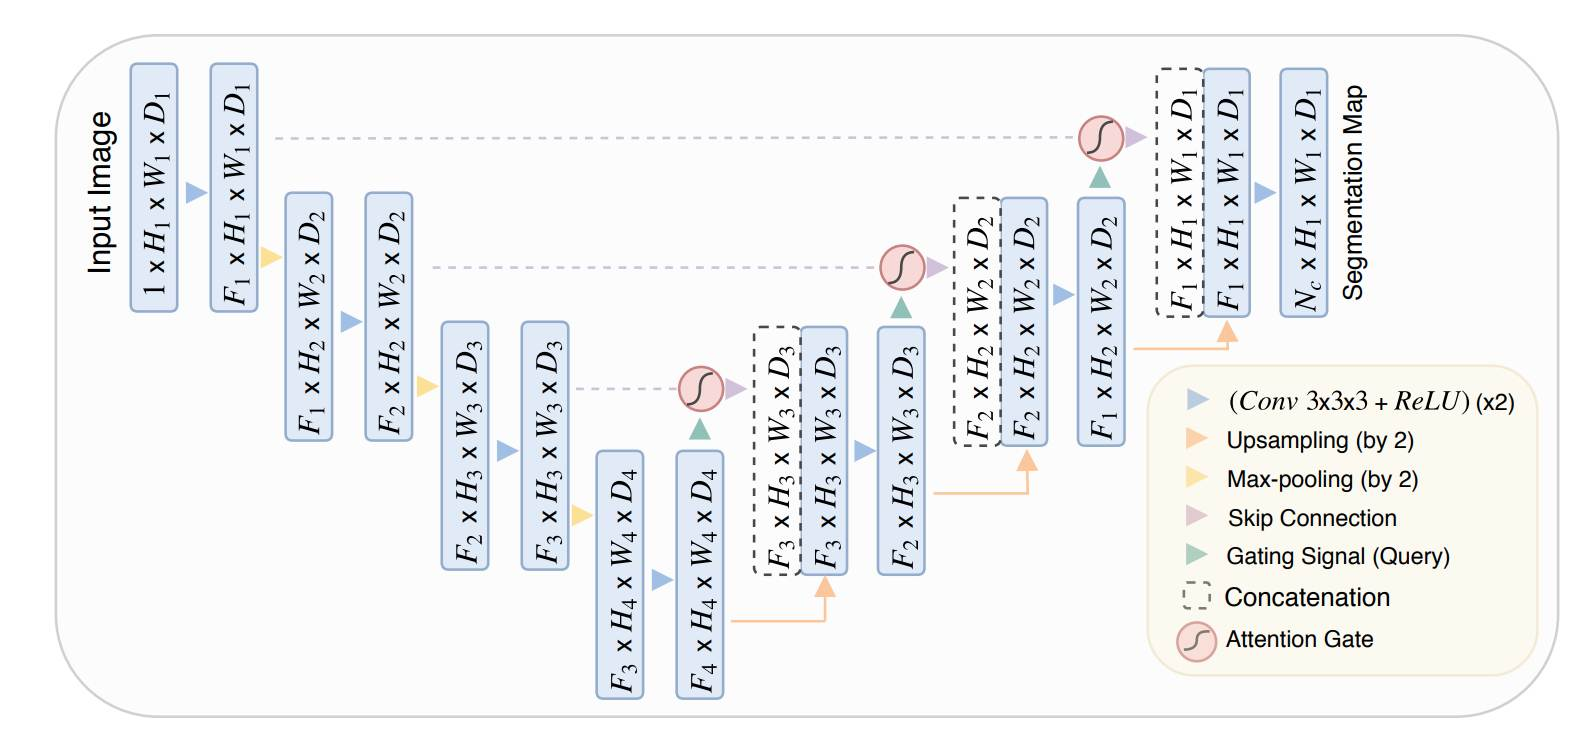
\includegraphics[width=.8\textwidth]{images/2025-07-22-14-33-52.png} 
    \caption{Shcema dell’Attention U-Net. Le frecce indicano il flusso di informazioni tra i moduli di encoder e decoder, con l’integrazione del modulo di attenzione.}
    \label{fig:attention_unet}
 \end{figure} 
Dal punto di vista implementativo, il modulo di attenzione riceve in input due segnali: da un lato, \textbf{le feature provenienti dal livello encoder} (contenenti informazione spaziale locale); dall’altro, \textbf{i segnali di gating dal decoder} (contenenti informazione semantica più astratta). L’interazione tra questi due flussi genera una \textbf{mappa di attenzione}, applicata tramite moltiplicazione ai tensori encoder, prima della loro trasmissione al decoder. In questo modo, il decoder riceve solo le informazioni più rilevanti per la predizione finale.

Nel contesto del presente lavoro, \textbf{nonostante un aumento moderato della complessità computazionale}, il modello \hlight{ha mostrato buone performance}, raggiungendo un \hlight{Dice score pari a 0.8415} nell’esperimento dedicato.

\Section{Esperimento Finale}

Il punto culminante di questa fase è stato rappresentato dall’esperimento \textbf{21}, in cui è stata utilizzata una \hlight{U-Net profonda con cinque livelli e stride finale lungo l’asse z pari a 1}. L’input adottava una ROI size tridimensionale pari a $(512, 512, 8)$, e il training è stato prolungato fino a \hlight{200 epoche} \ref{fig:losses}. 

\begin{minipage}{.48\textwidth}
    \begin{figure}[H] 
        \centering 
        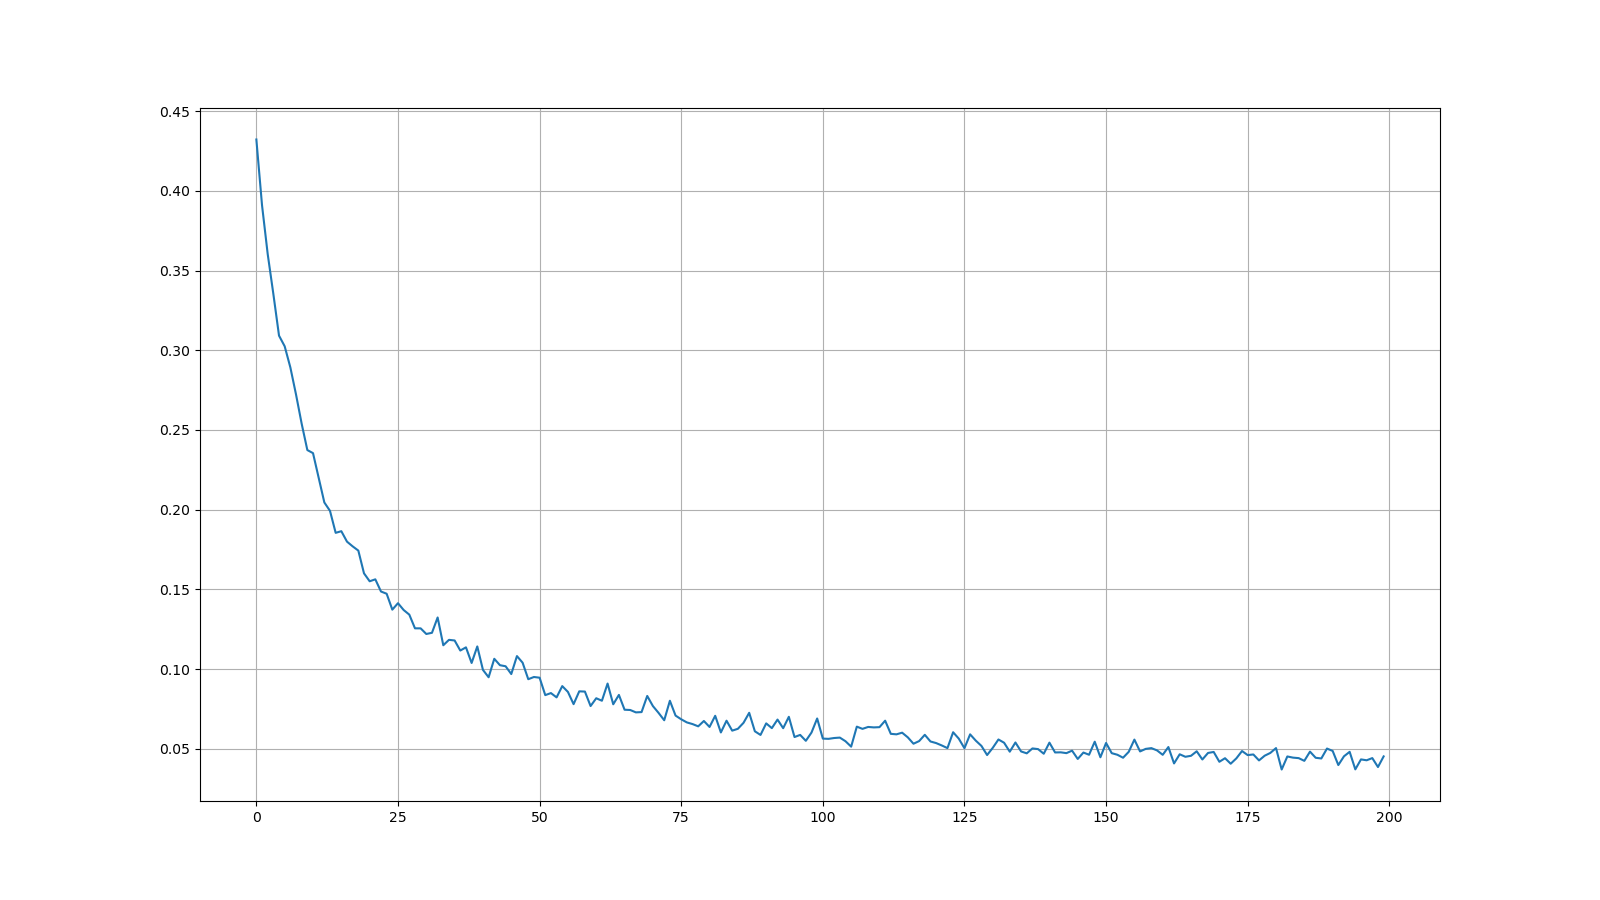
\includegraphics[width=\textwidth]{figures/losses.png} 
        \caption{Andamento delle funzioni di loss durante il training dell’esperimento finale(EXP 21).}
        \label{fig:losses}
    \end{figure} 
\end{minipage}
\hfill
\begin{minipage}{.48\textwidth}
    \begin{figure}[H] 
        \centering 
        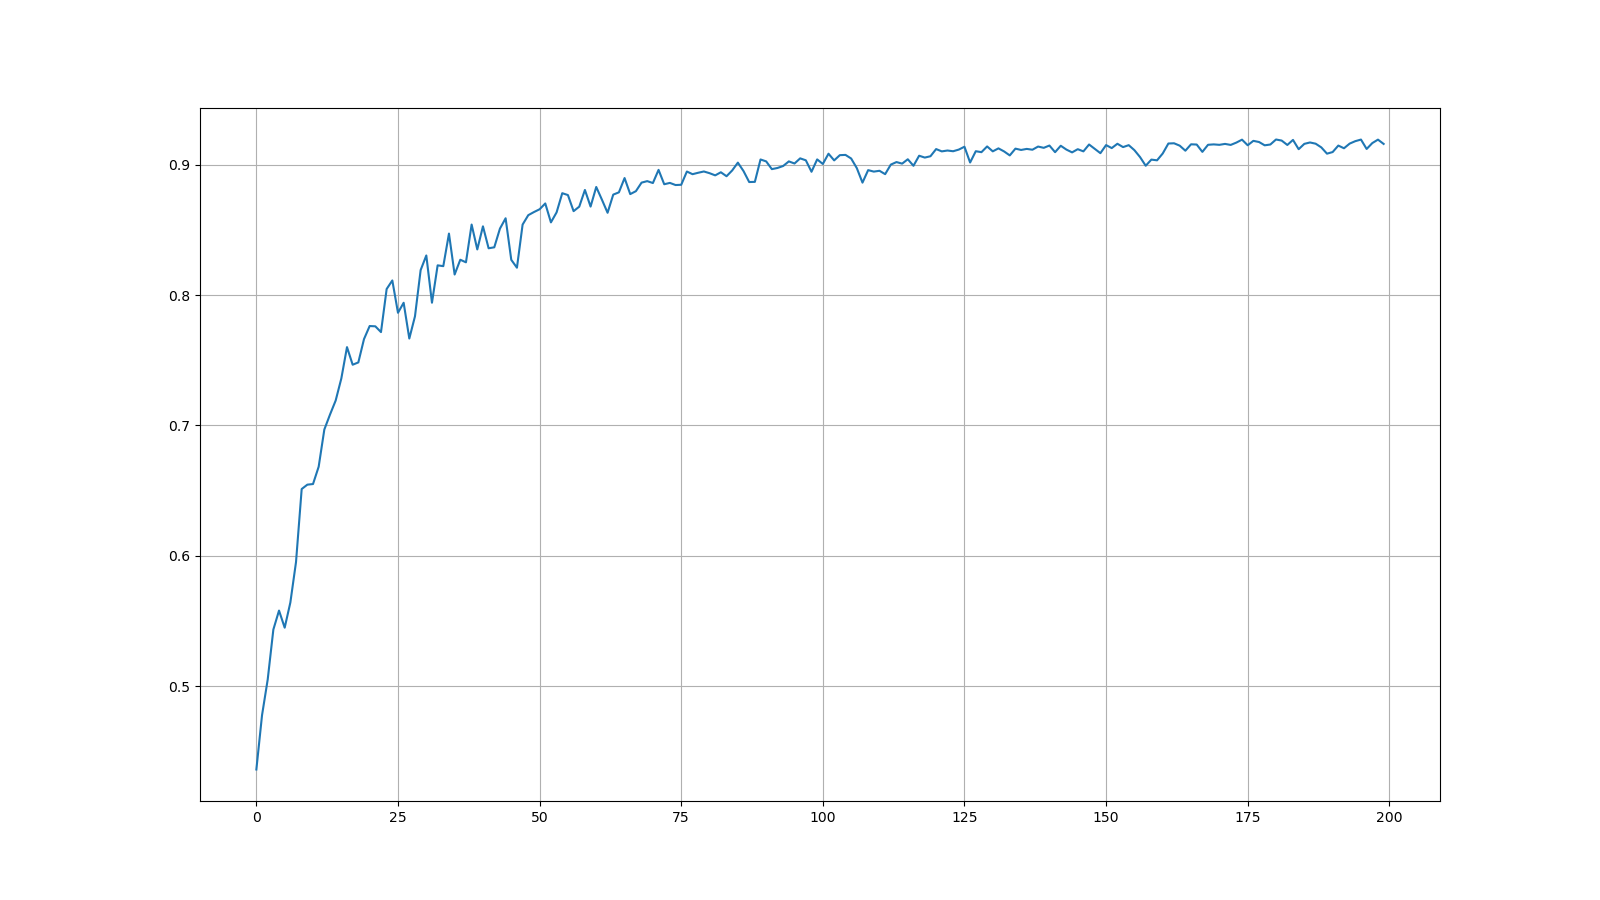
\includegraphics[width=\textwidth]{figures/metrics.png} 
        \caption{Andamento delle metriche di valutazione durante il training dell’esperimento finale(EXP 21).}
        \label{fig:metrics}
    \end{figure} 
\end{minipage}




In queste condizioni, \hlight{il modello ha raggiunto un Dice score pari a 0.9124} \ref{fig:metrics}, \hlight{il valore più alto registrato su tutto il test set} \ref{fig:final_segmentation_examples}. Questo risultato rappresenta non solo il successo di una specifica configurazione, ma anche la validazione dell’intero \textbf{processo di ottimizzazione}, culminato in un \textbf{modello accurato}, \textbf{robusto} e valutato con \textbf{criteri metodologicamente solidi}.


\begin{table}[H]
\centering
\begin{NiceTabular}{rlccc}[rules/color={gray!85},rules/width=0.8pt]
\CodeBefore
\rowcolors{1}{}{gray!3}
\Body
\toprule
\textbf{EXP} & \textbf{Configurazione} & \textbf{Dice} & \textbf{$\Delta$} & \textbf{Note} \\
\midrule
16 & Config. originale & 0.8863 & \color{red}{-3.3\%} & Sovrastima precedente \\
20 & Stessa config. + val. rigorosa & 0.8567 & \color{gray}{0\%} & Benchmark corretto \\
19 & Attention U-Net & 0.8415 & \color{red}{-1.8\%} vs 20 & Robustezza verificata \\
\rowcolor{blue!7}
21 & U-Net avanzato & 0.9124 & \color{teal}{+6.5\% vs 20} & Nuovo state-of-the-art \\
\bottomrule
\end{NiceTabular}
\caption{Analisi dettagliata dei risultati finali. La colonna $\Delta$ mostra: per EXP 16 la sovrastima rispetto alla nuova metodologia, per EXP 19-21 la variazione rispetto al benchmark corretto (EXP 20).}
\label{tab:final_results_detailed}
\end{table}



\begin{figure}[H]
    \centering
    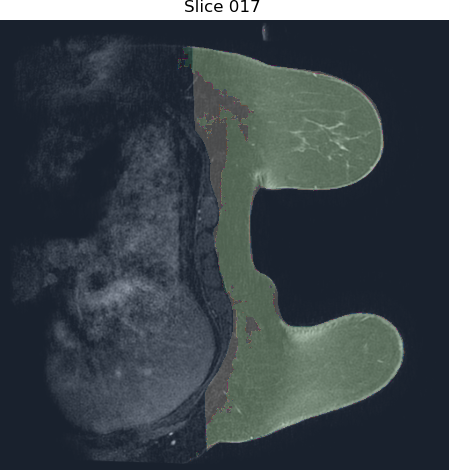
\includegraphics[width=0.40\textwidth]{figures/slice_017.png} 
    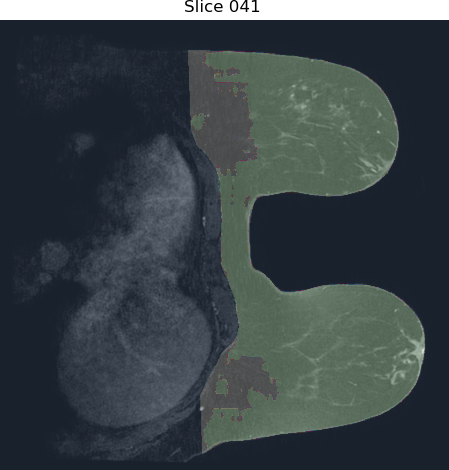
\includegraphics[width=0.40\textwidth]{figures/slice_041.png} 
    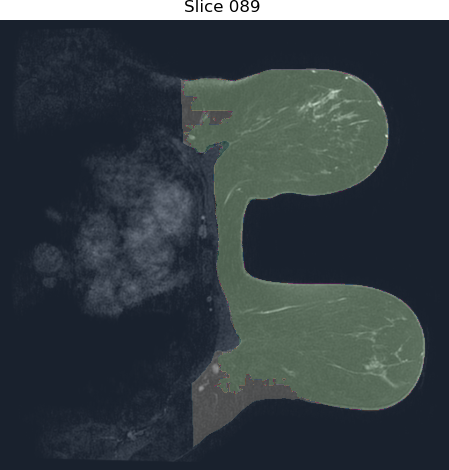
\includegraphics[width=0.40\textwidth]{figures/slice_089.png} 
    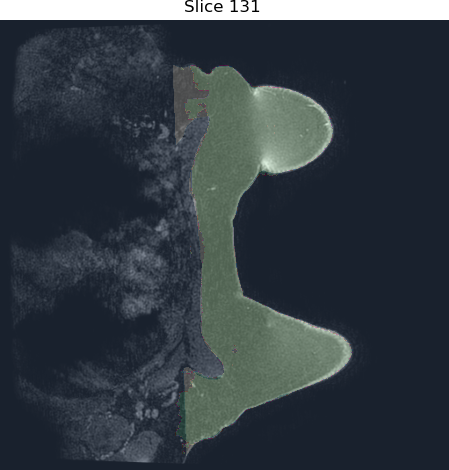
\includegraphics[width=0.40\textwidth]{figures/slice_131.png} 
    \caption{Esempi di segmentazione ottenuti con il modello finale (EXP 21). Le immagini mostrano le predizioni su diverse slice del test set, evidenziando la capacità del modello di identificare correttamente le aree di interesse.}
    \label{fig:final_segmentation_examples}
\end{figure}

\Subsection{Post-processing morfologico: operazione di Closing}

Al termine dell’addestramento del modello finale (EXP~21), è stata introdotta una fase opzionale di \textbf{post-processing morfologico} sulle maschere di segmentazione prodotte, con l’obiettivo di correggere eventuali discontinuità e imperfezioni residue lungo i margini delle strutture segmentate.

L’operazione applicata è il \textbf{closing morfologico} (\emph{dilatazione seguita da erosione}). Questo tipo di trasformazione è comunemente utilizzato per \textbf{colmare piccoli vuoti} all’interno delle regioni segmentate, \textbf{uniformare i bordi} delle maschere e \textbf{migliorare la connettività} delle strutture anatomiche in presenza di interruzioni puntuali.


L'implementazione è stata realizzata creando una funzione custom in Python che applica il closing morfologico su ciascuna maschera di segmentazione generata dal modello. La funzione utilizza la libreria \texttt{scikit-image} per eseguire le operazioni morfologiche, specificando un \textbf{kernel di dimensione fissata dal parametro in ingresso}:

\begin{code}{python}
from scipy.ndimage import binary_closing
from monai.transforms import MapTransform
import torch
import numpy as np

class MorphologicalClosing():
    def __init__(self, dim=12):
        self.dim = dim
        self.structure = np.ones((self.dim, self.dim, self.dim), dtype=bool)
    def __call__(self, x):
        device = x.device if isinstance(x, torch.Tensor) else torch.device('cpu')
        # convert to numpy
        if isinstance(x, torch.Tensor):
            x = x.cpu().numpy()
        # remove first dimension
        x = x.squeeze(0) if x.ndim > 3 else x
        closed_np = binary_closing(x, structure=self.structure)
        # re-add first dimension
        closed_np = closed_np[None, ...]
        # convert back to tensor and move to original device
        closed_tensor = torch.tensor(closed_np, dtype=torch.float32, 
                                    device=device)
        return closed_tensor
\end{code}
Sono state testate diverse dimensioni per il \textbf{kernel size} dell’operazione di closing, variando il parametro tra valori compresi tra 6 e 16. L’analisi sistematica ha mostrato che la dimensione ottimale era pari a \hlight{10}, che garantiva il miglior compromesso tra \textbf{uniformità dei bordi} e \textbf{preservazione dei dettagli anatomici}, evitando sia un’eccessiva erosione sia la formazione di artefatti.

\begin{figure}[H] 
  	\centering 
 	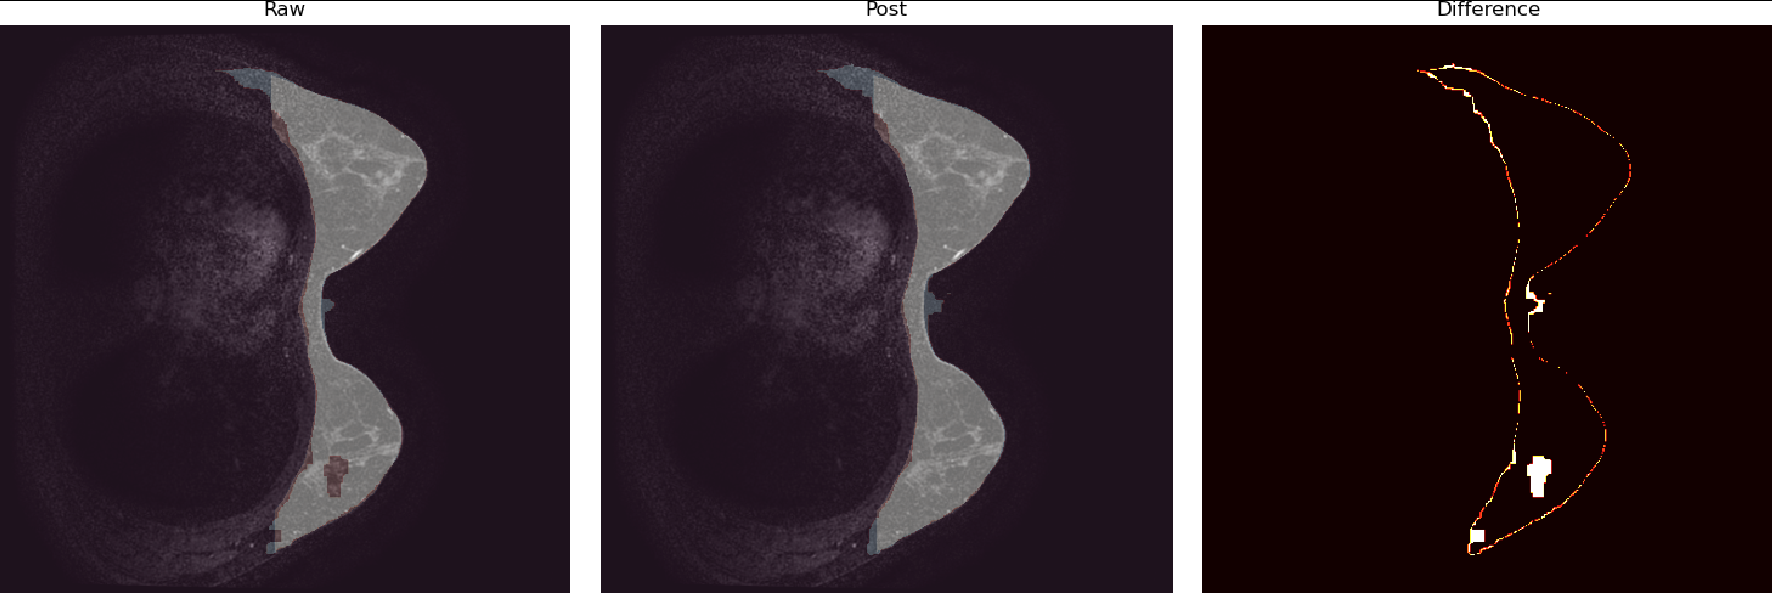
\includegraphics[width=\textwidth]{images/2025-08-08-18-52-24.png} 
    \caption{Esempio di segmentazione prima e dopo l'applicazione del closing morfologico. Le immagini mostrano come il closing migliori la coesione delle strutture segmentate, eliminando piccole discontinuità e rendendo le maschere più uniformi.}
    \label{fig:closing_example}
 \end{figure} 

L’effetto del closing \ref{fig:closing_example} è stato valutato rieseguendo la metrica di \textbf{Dice score} sul \emph{test set}. Il modello finale, che in fase di validazione rigorosa aveva raggiunto un valore di \textbf{0.9124}, \hlight{ha beneficiato di un incremento fino a 0.9161} dopo il post-processing. Questo risultato conferma che, pur trattandosi di un miglioramento numericamente modesto \textbf{(\(+0.0037\)),} \hlight{l’operazione di closing ha contribuito a rifinire ulteriormente le maschere, portando a un output visivamente più coerente e clinicamente più fruibile.}



